\documentclass[../main.tex]{subfiles}

\begin{document}
\newpage
\thispagestyle{empty}
\begin{center}
    {
\includegraphics[width=0.5\textwidth]{Imagenes/Logo UMA.jpg}\par}
    \vspace{1cm}
    {\bfseries\LARGE \Facultad \par}
    \vspace{0.5cm}
    {\scshape\Large \Grado \par}
    \vspace{3cm}
    {\scshape\Huge Planos \par}
    \vspace{1.5cm}
    {\itshape\Large \TituloProyecto \par}
    \vfill
    {\Large Solicitante: \par}
    {\Large \Solicitante  \par}
    \vspace{1cm}
    {\Large Autores: \par}
    {\Large \Autora \par}
    {\Large \Autor \par}
    \vfill
    {\Large \Fecha \par}
\end{center}

% El documento que contiene los planos se iniciará con un índice que hará referencia a cada uno de ellos, indicando su ubicación, con el fin de facilitar su utilización.
\chapter*{Índice de planos:}
\tableof{Planos}
\toftagstart{Planos}
% Contendrán la información gráfica, alfanumérica, de códigos y de escala, necesaria para su comprensión.

% Plano Situación (lo mismo que el de abajo pero desde un poquillo más lejos)
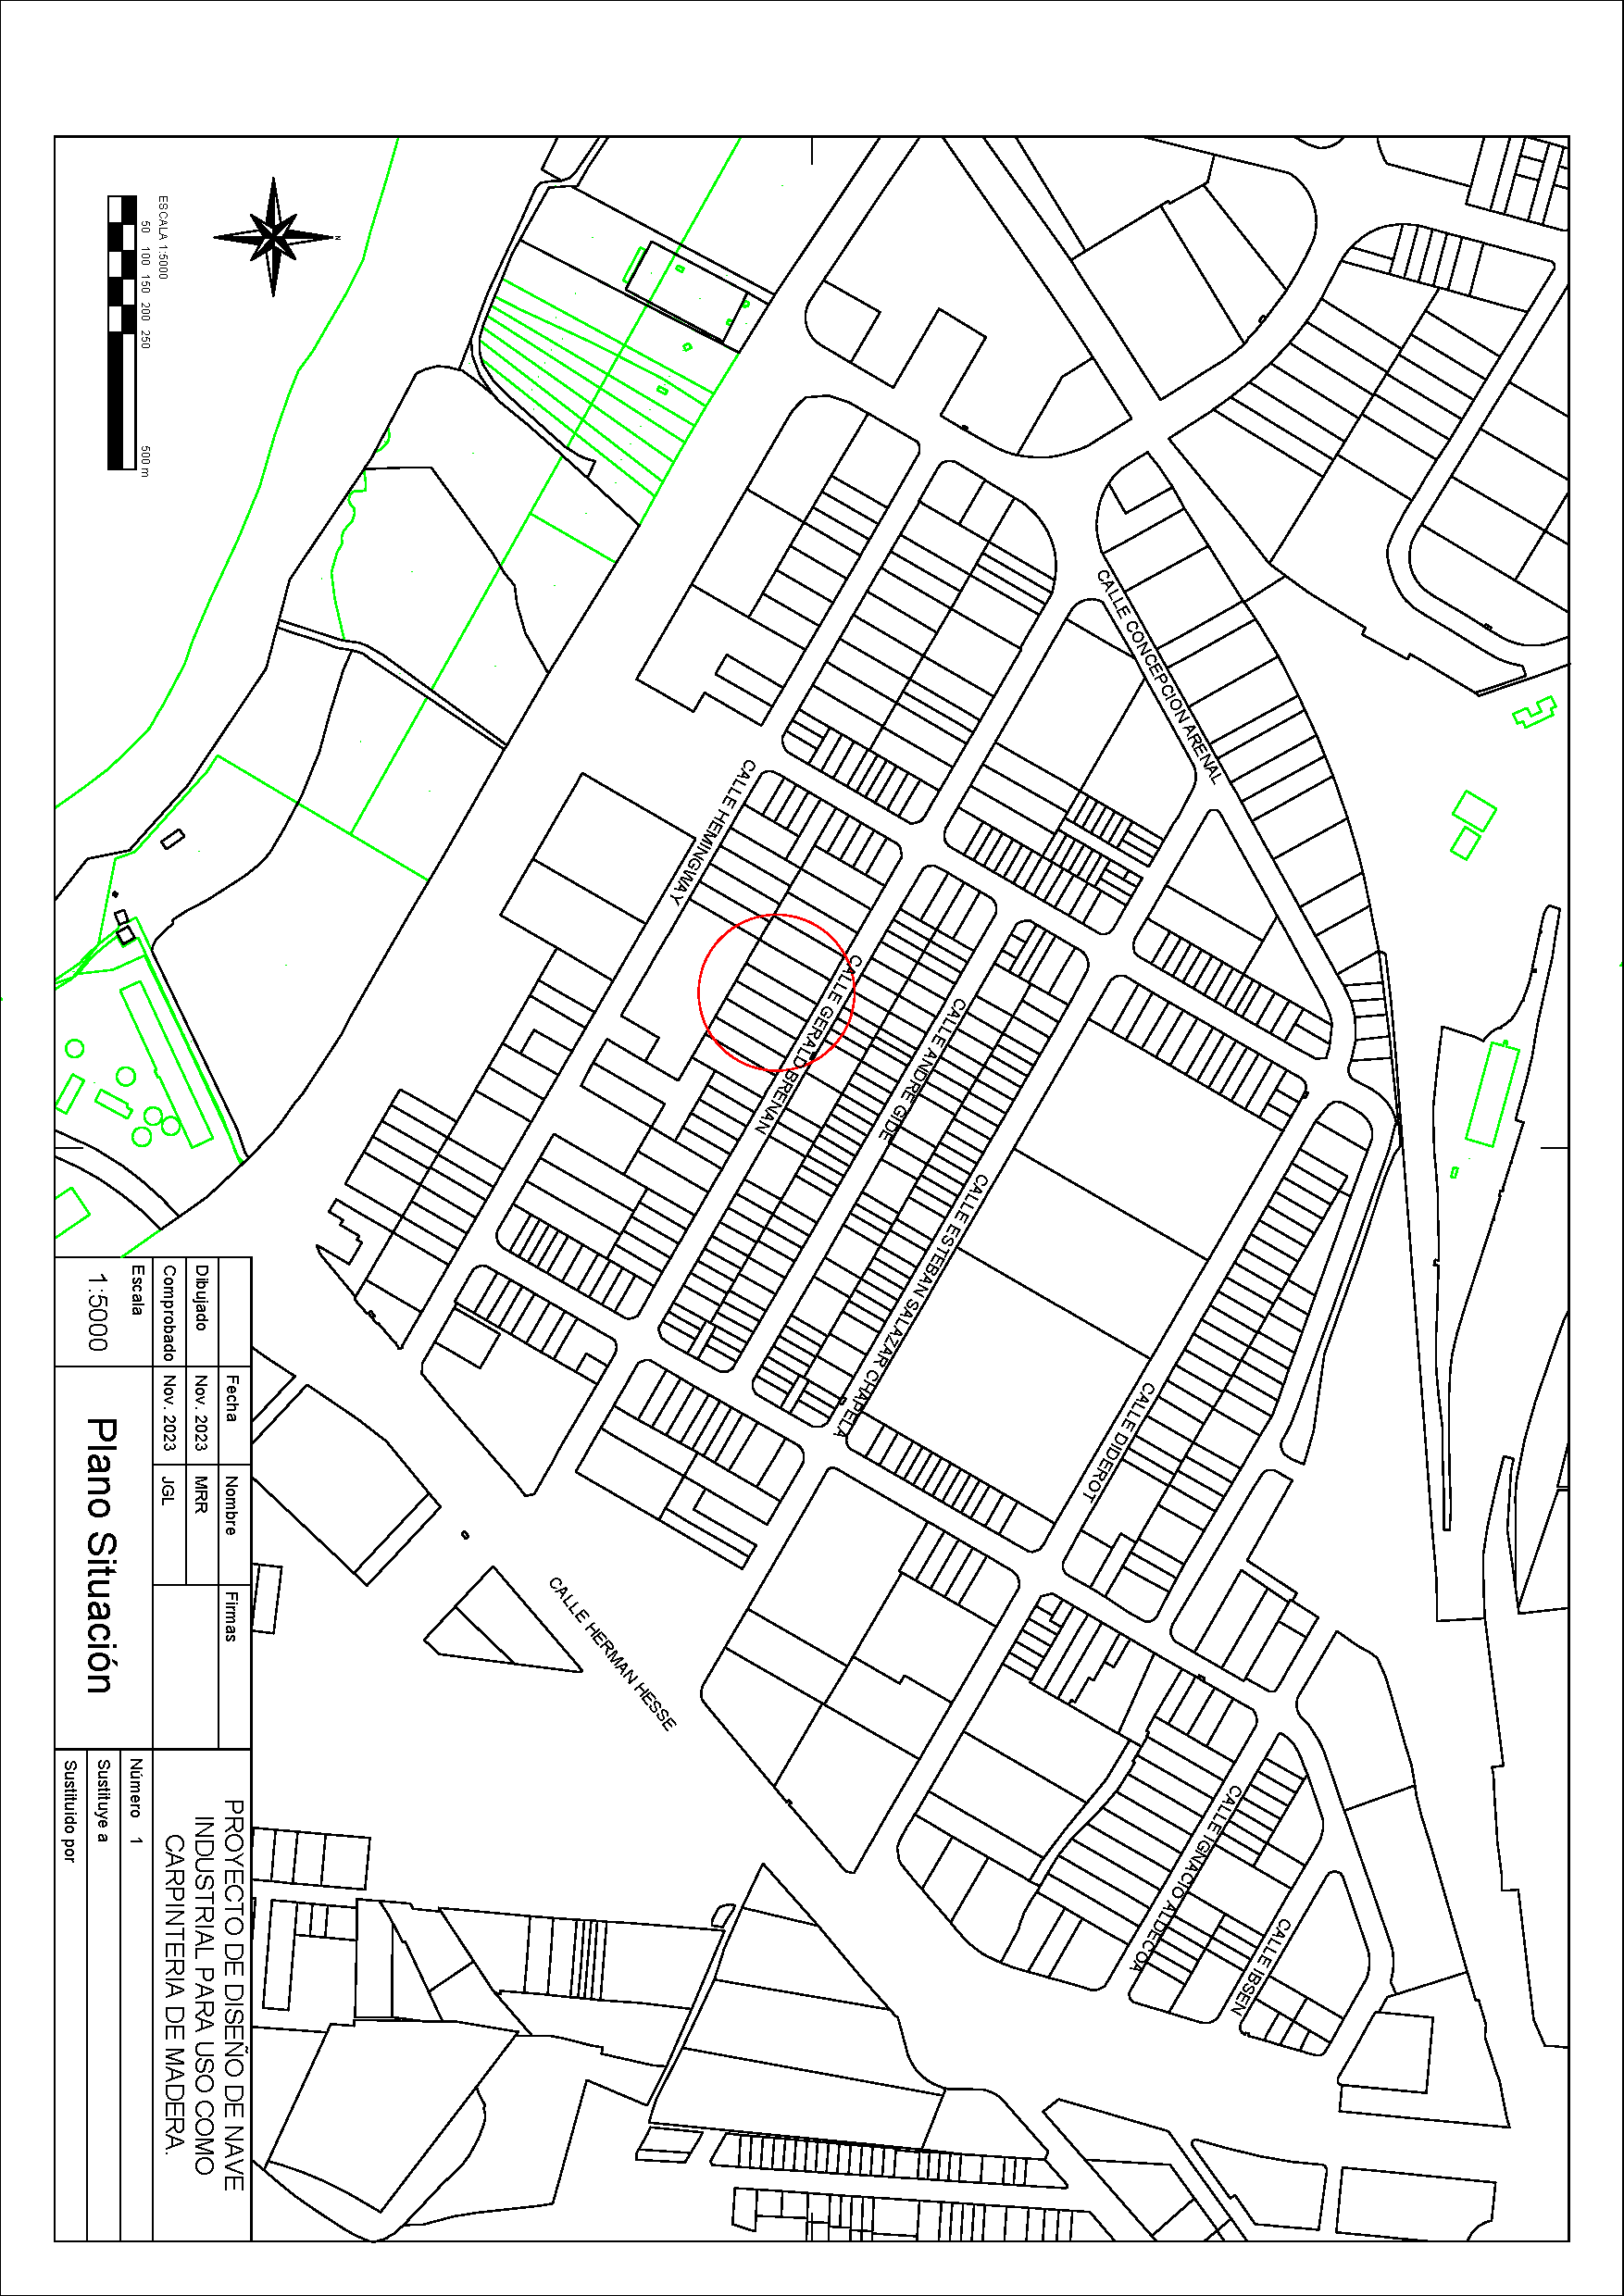
\includepdf[pages={1},pagecommand={
    \thispagestyle{empty}
    \addcontentsline{toc}{section}{Plano 1: Plano Situación}}]{Planos/Plano Situacion.pdf}
    
% Plano Emplazamiento (lo del catastro pero en bonito)
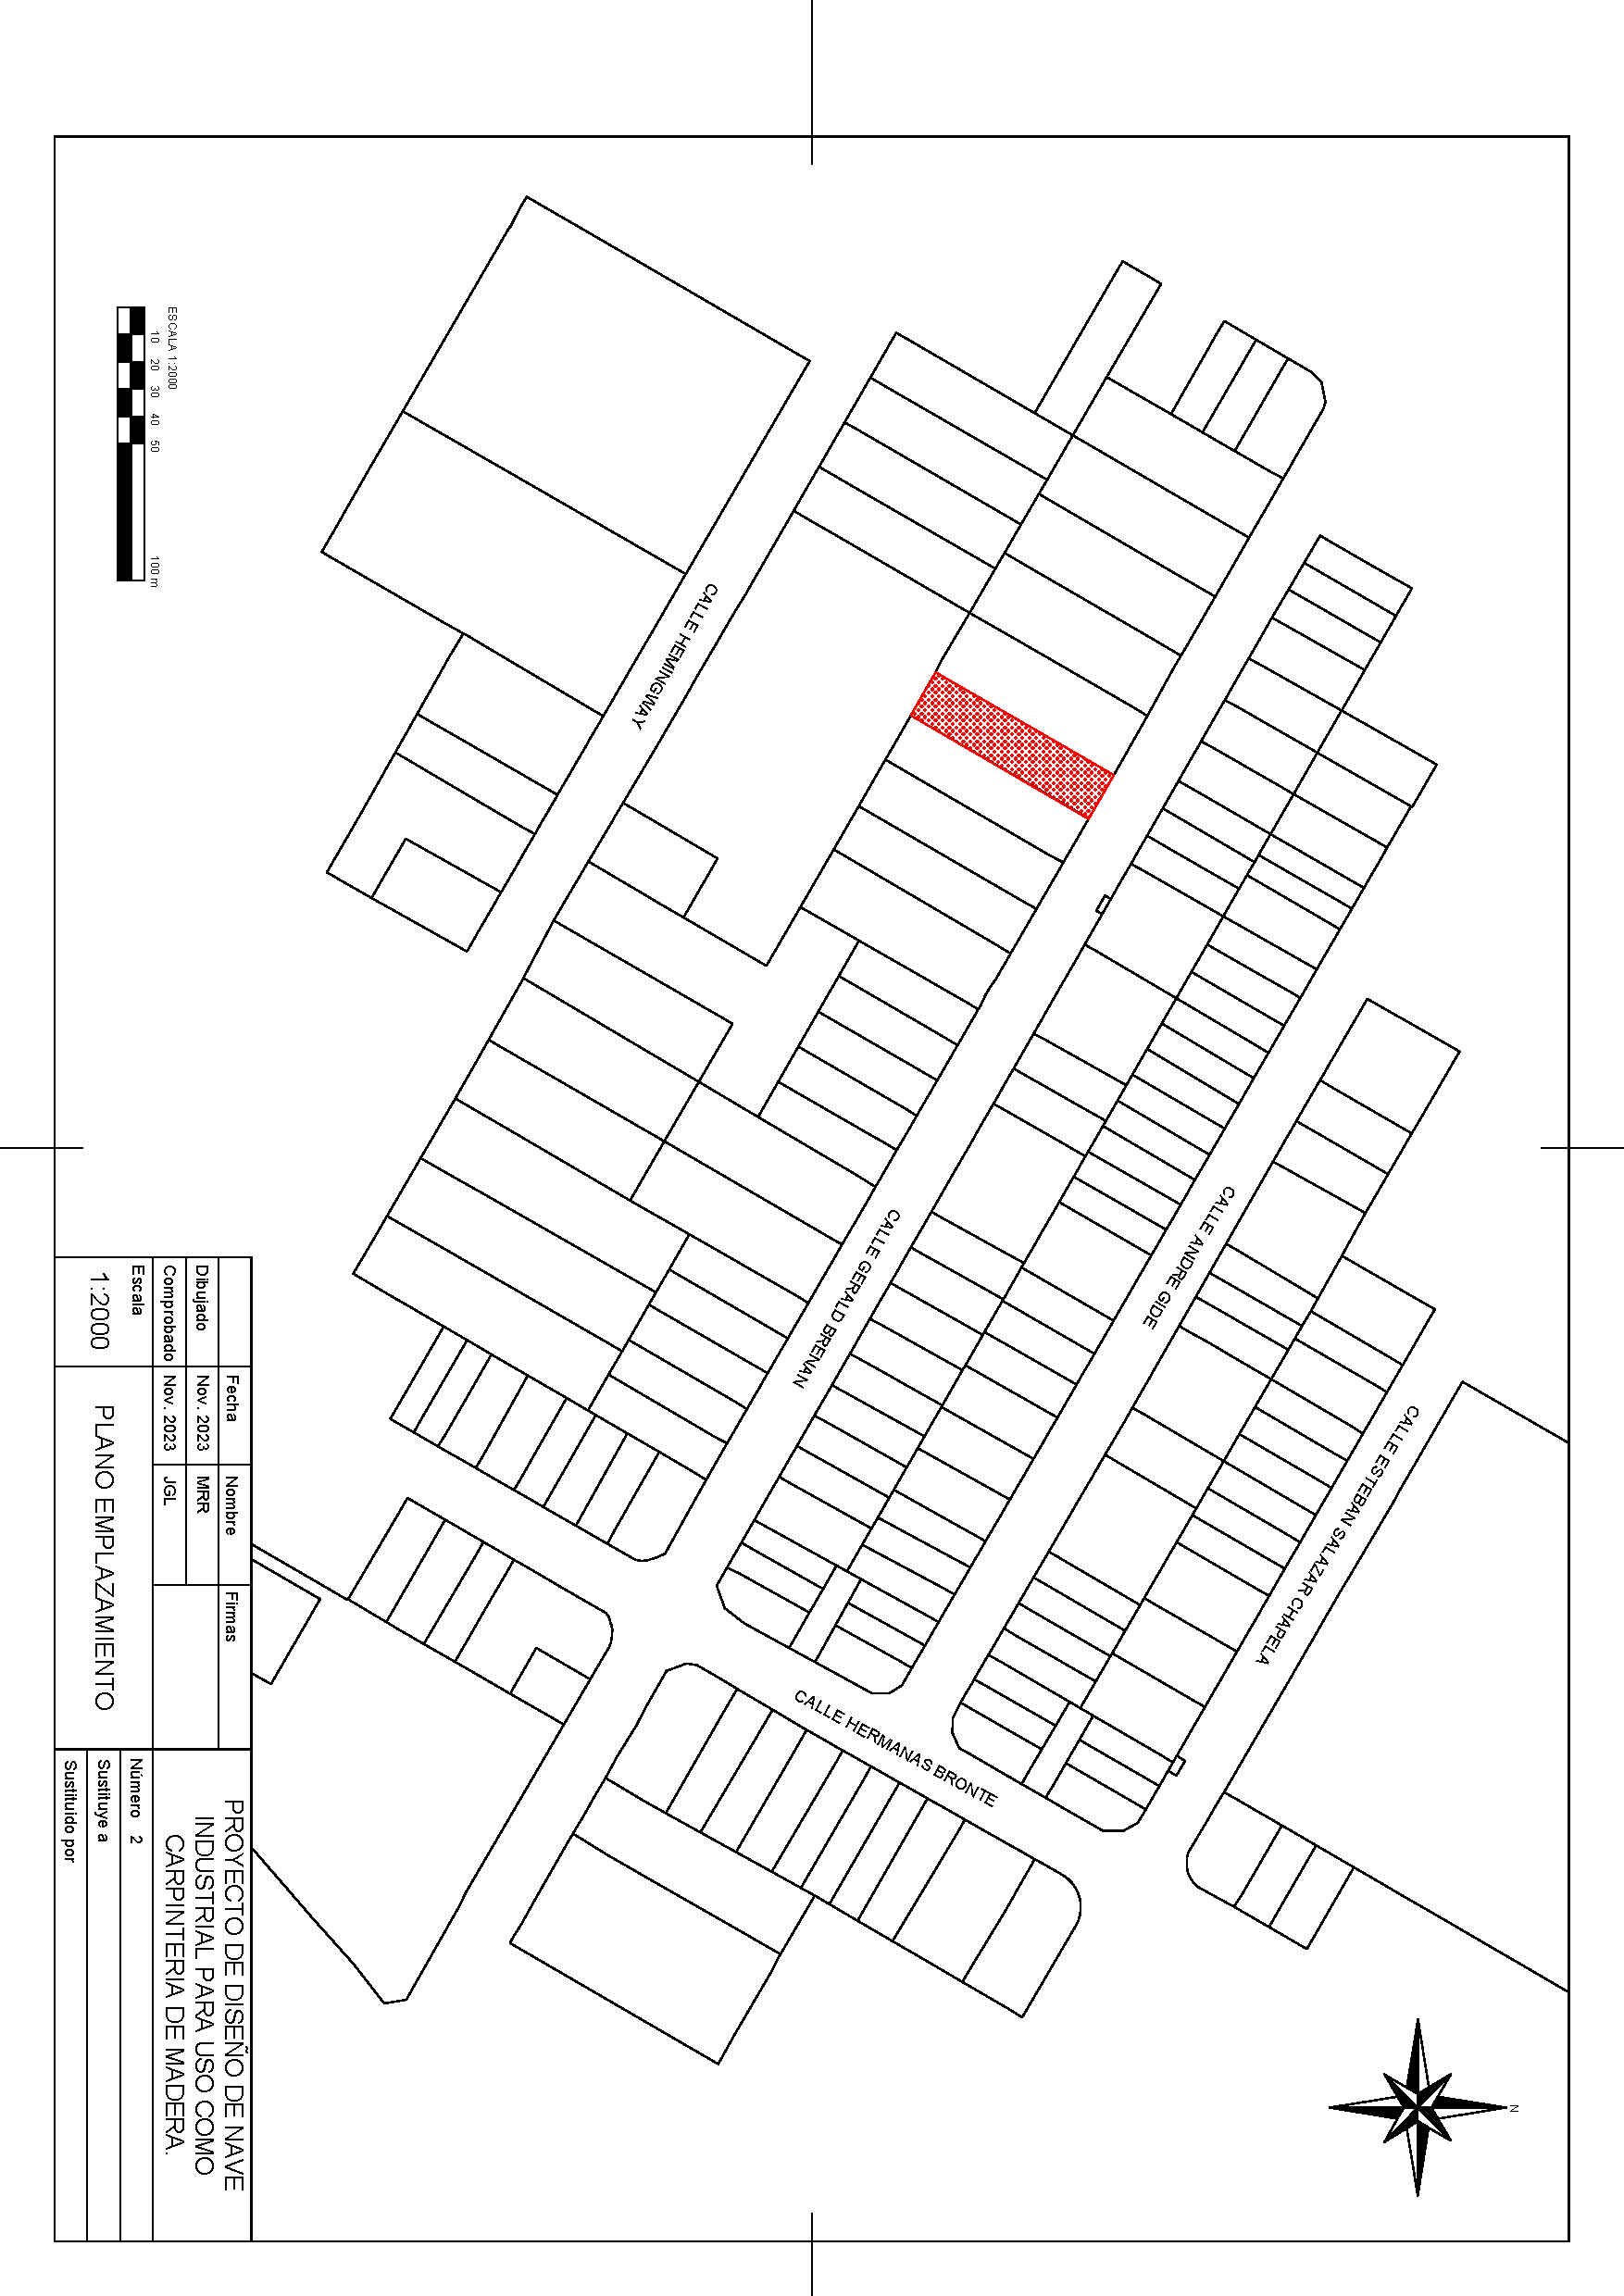
\includepdf[pages={1},pagecommand={
    \thispagestyle{empty}
    \addcontentsline{toc}{section}{Plano 2: Plano Emplazamiento}}]{Planos/Plano Emplazamiento.pdf}
    
% Distribución General (lo del autocad)
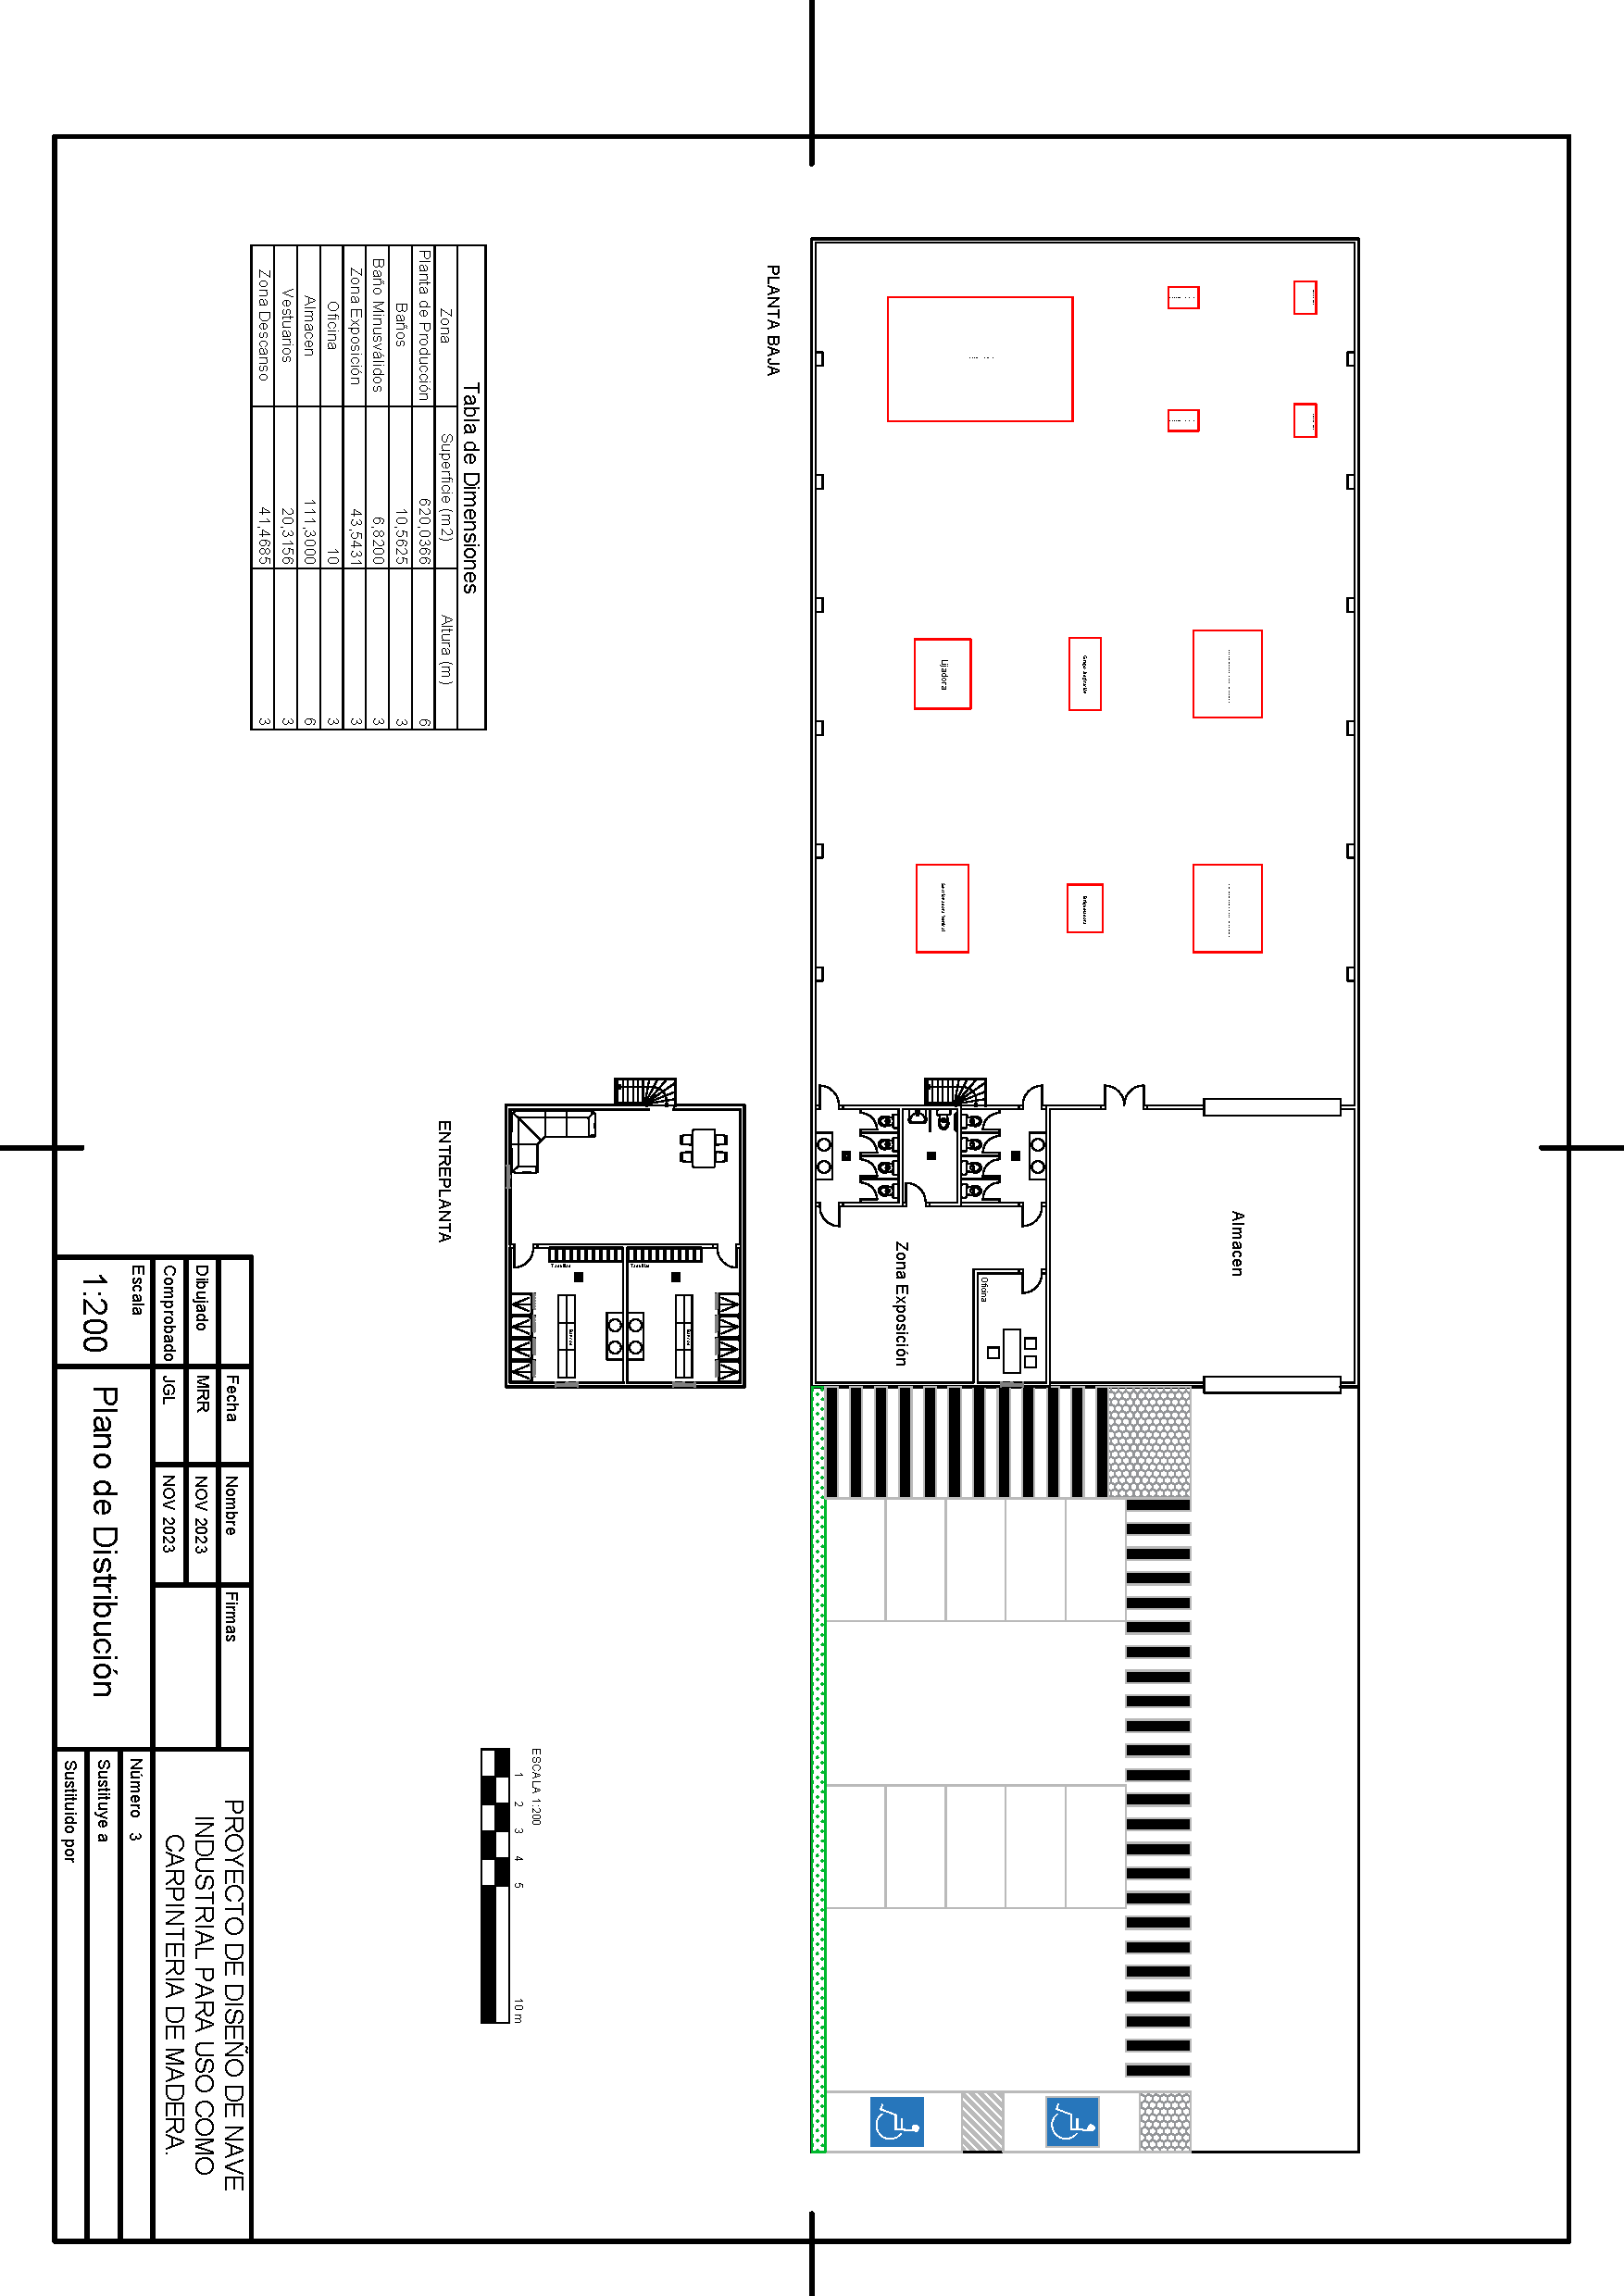
\includepdf[pages={1},pagecommand={
    \thispagestyle{empty}
    \addcontentsline{toc}{section}{Plano 3: Plano de Distribución General}}]{Planos/Plano General de Distribucion.pdf}
    
% Fontanería
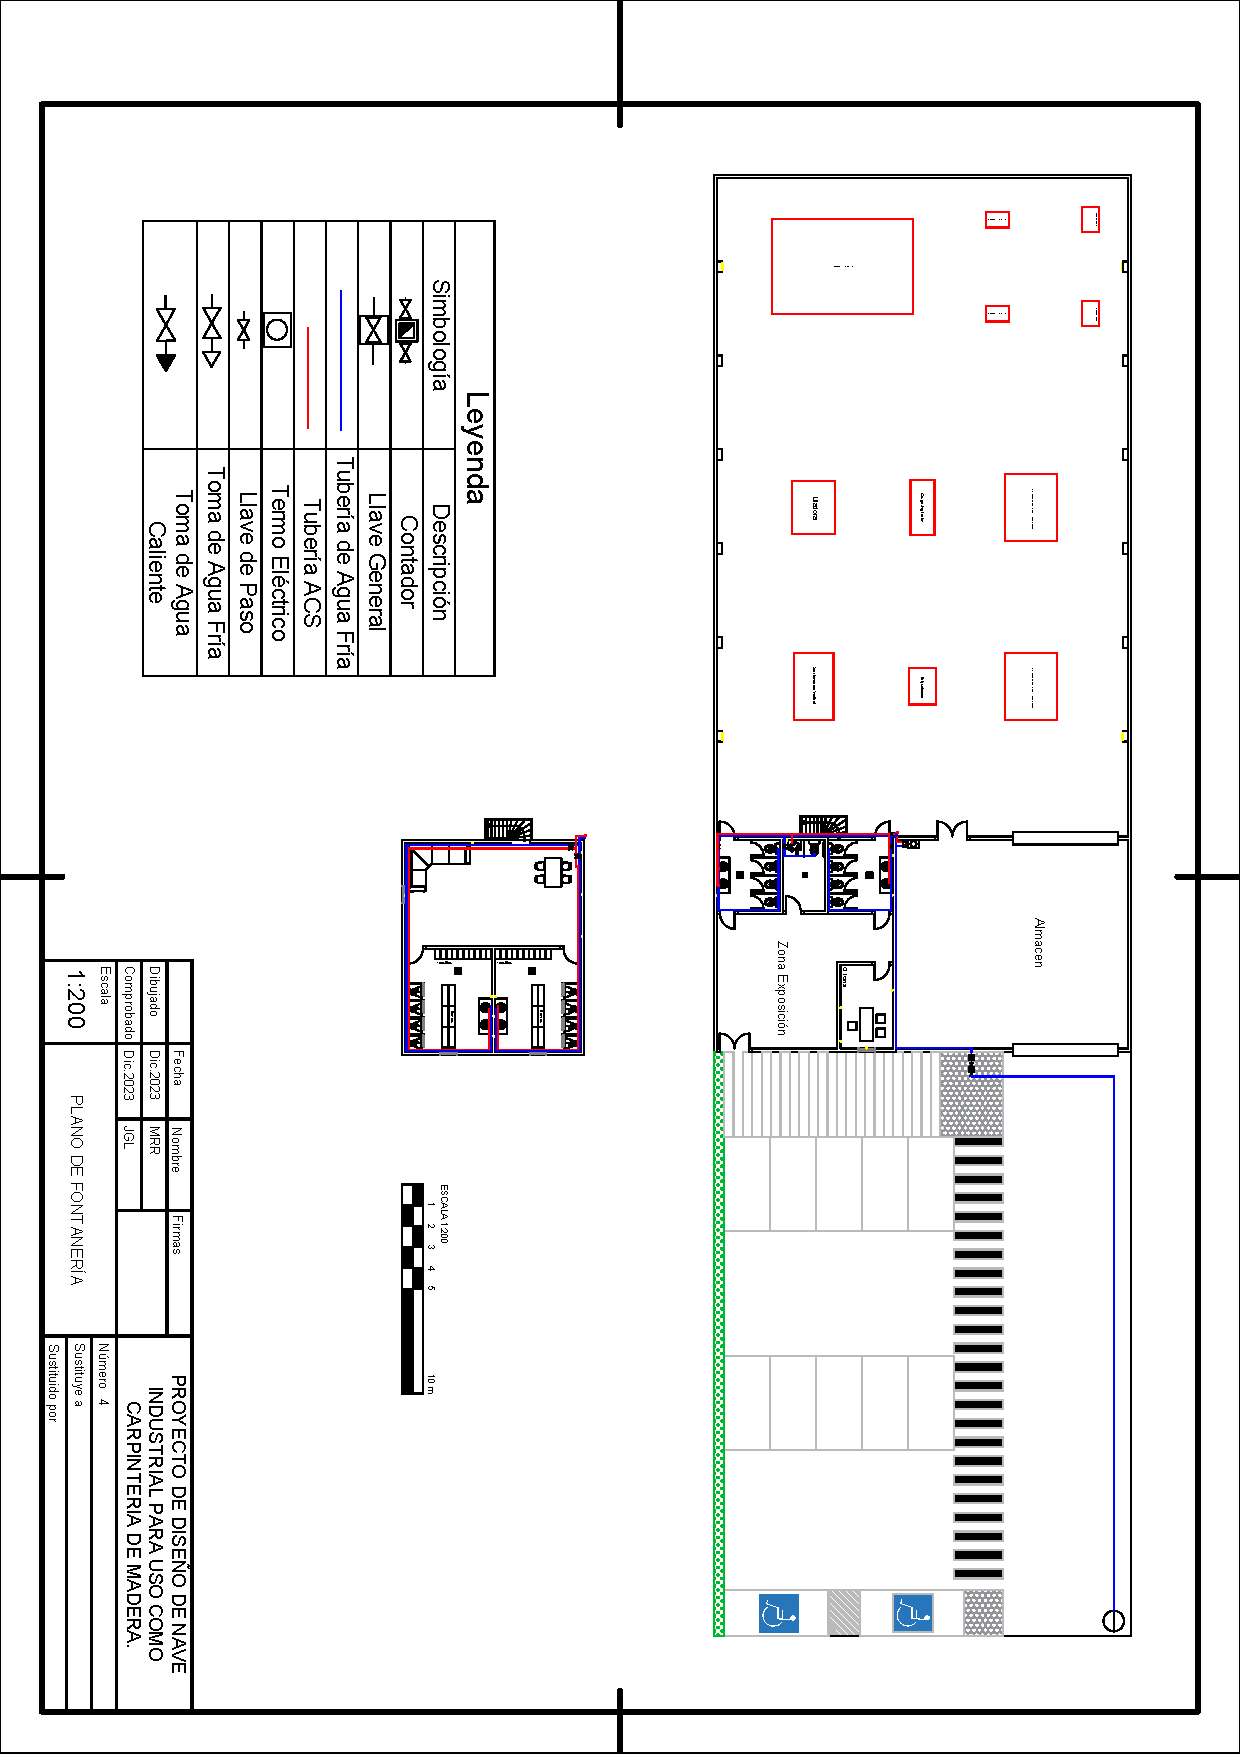
\includepdf[pages={1},pagecommand={
    \thispagestyle{empty}
    \addcontentsline{toc}{section}{Plano 4: Plano Instalación de Fontanería}}]{Planos/Plano Fontaneria.pdf}
    
% Saneamiento (Plubiales)

% Saneamiento (Residuales)

% Luminarias
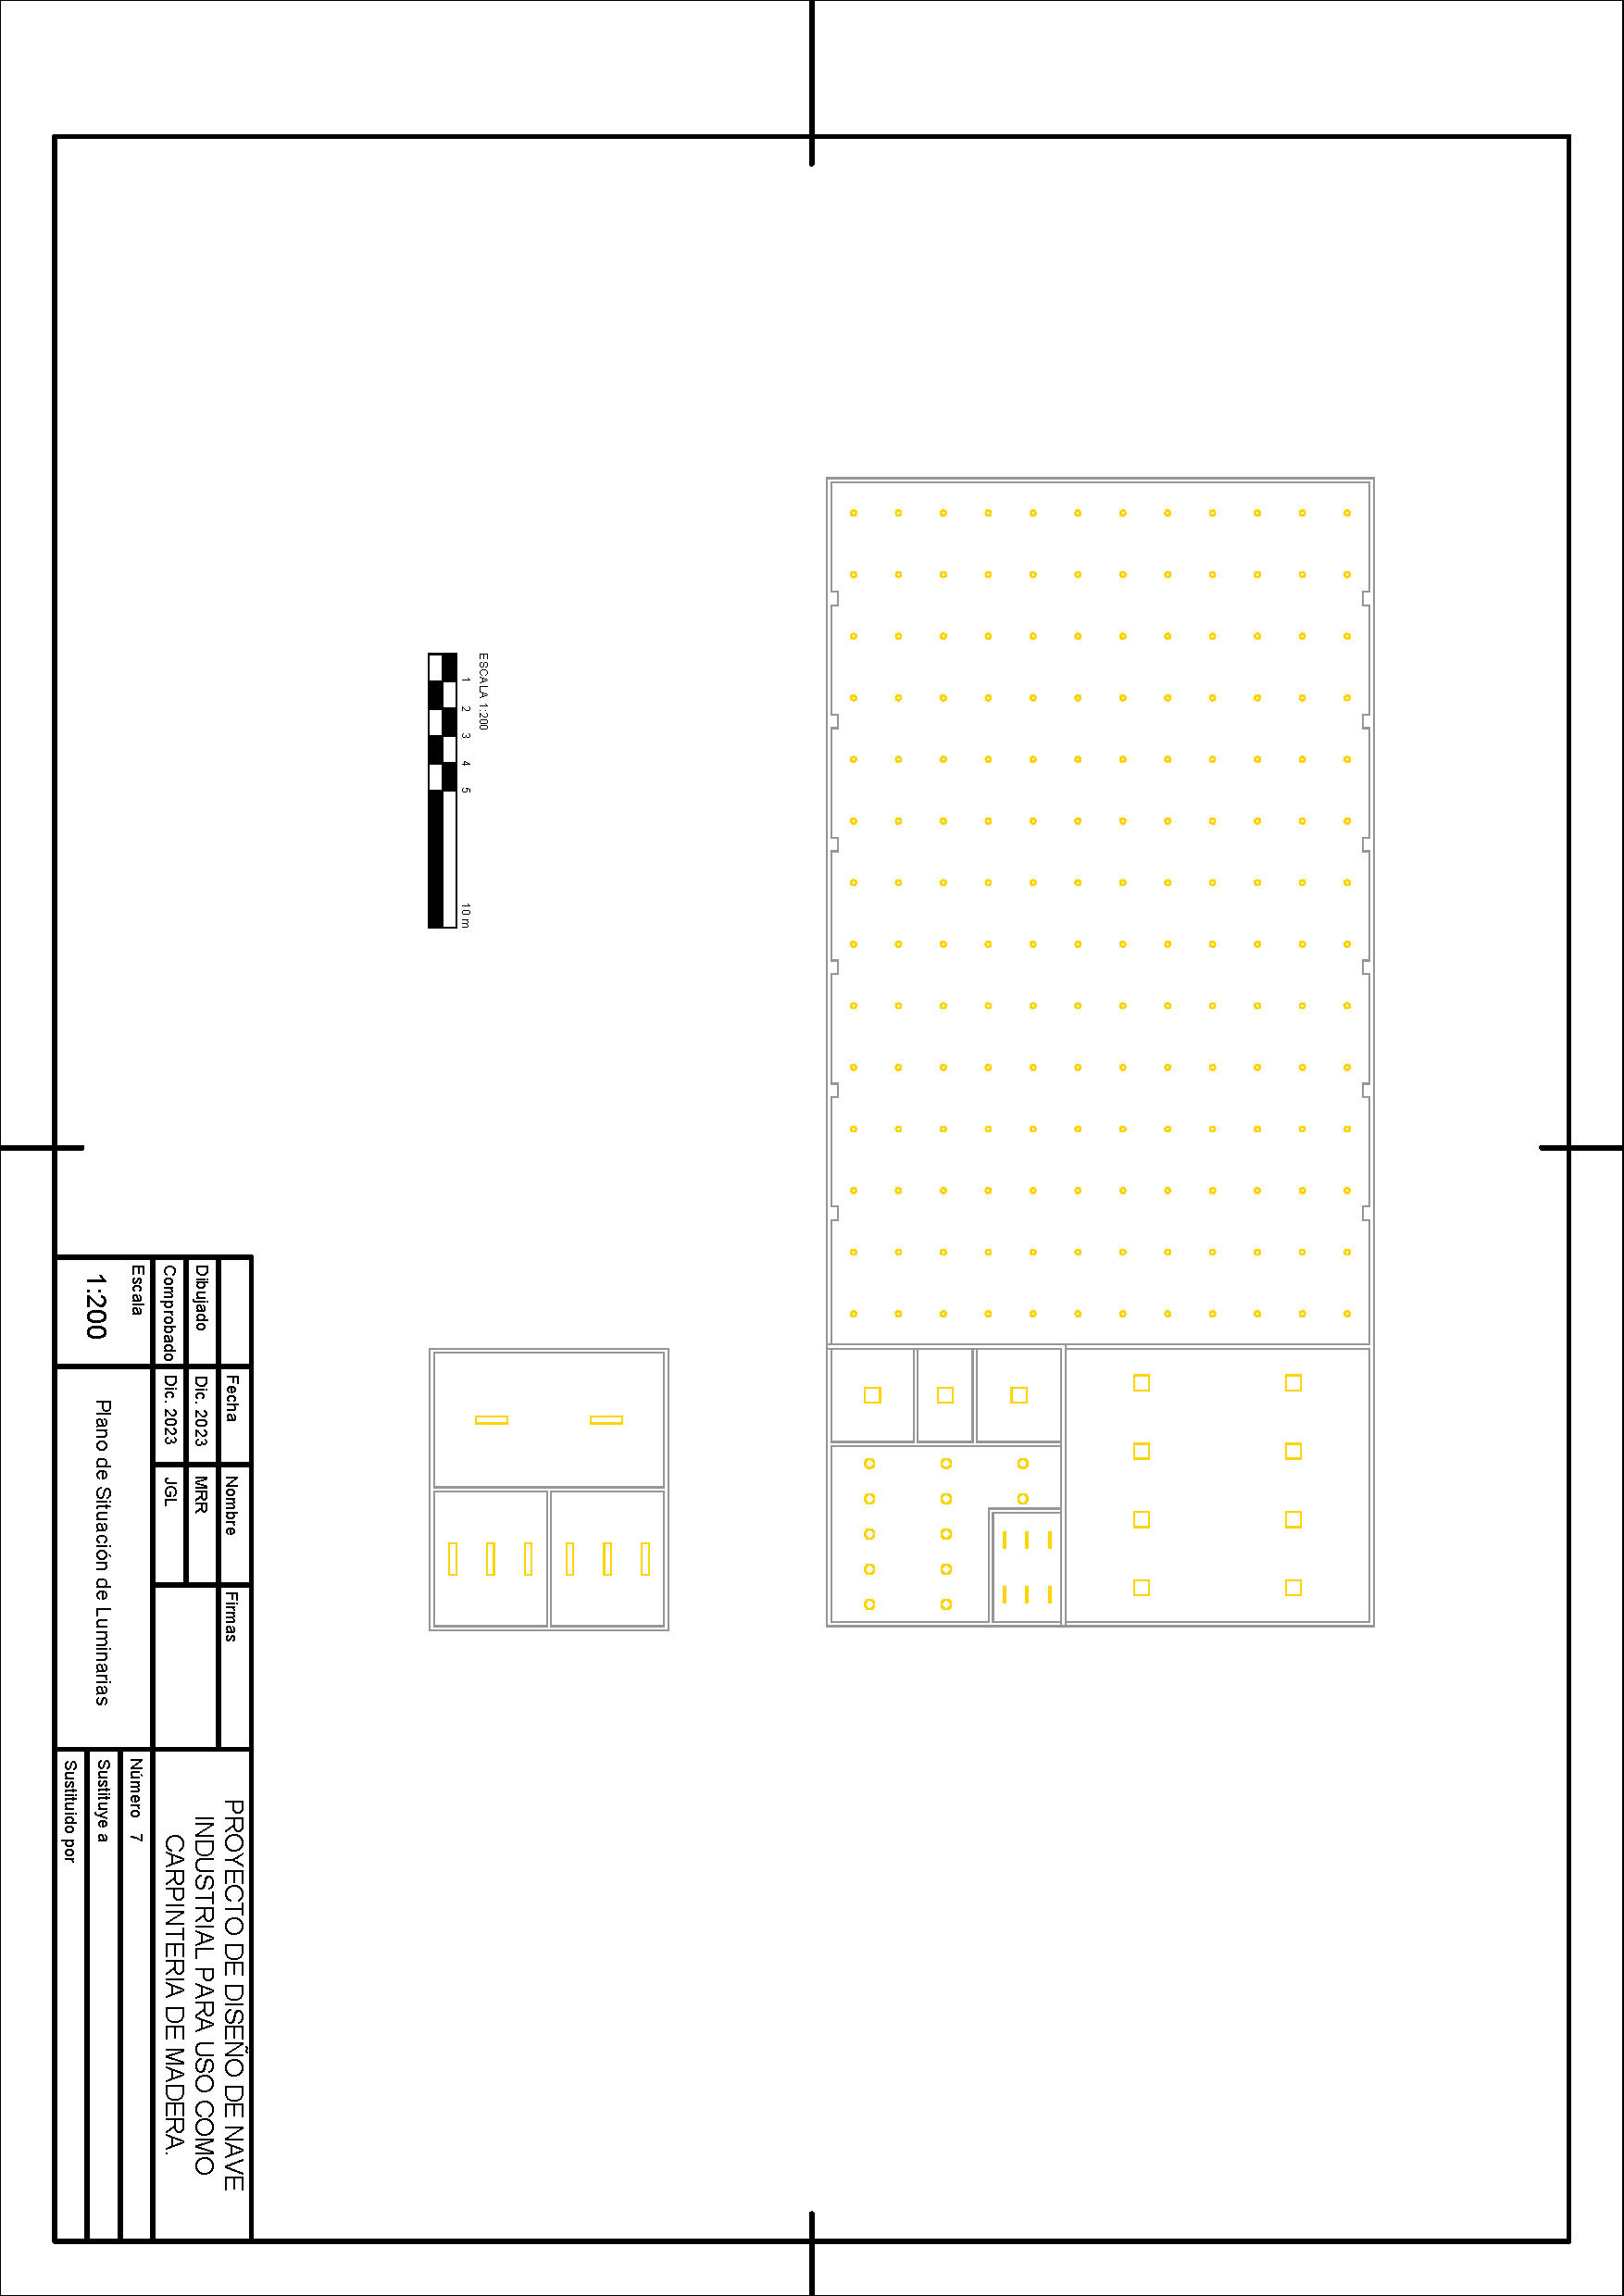
\includepdf[pages={1},pagecommand={
    \thispagestyle{empty}
    \addcontentsline{toc}{section}{Plano 7: Plano Instalación de Iluminación: Luminarias}}]{Planos/Plano Luminarias.pdf}
    
% Parámetros Lumínicos
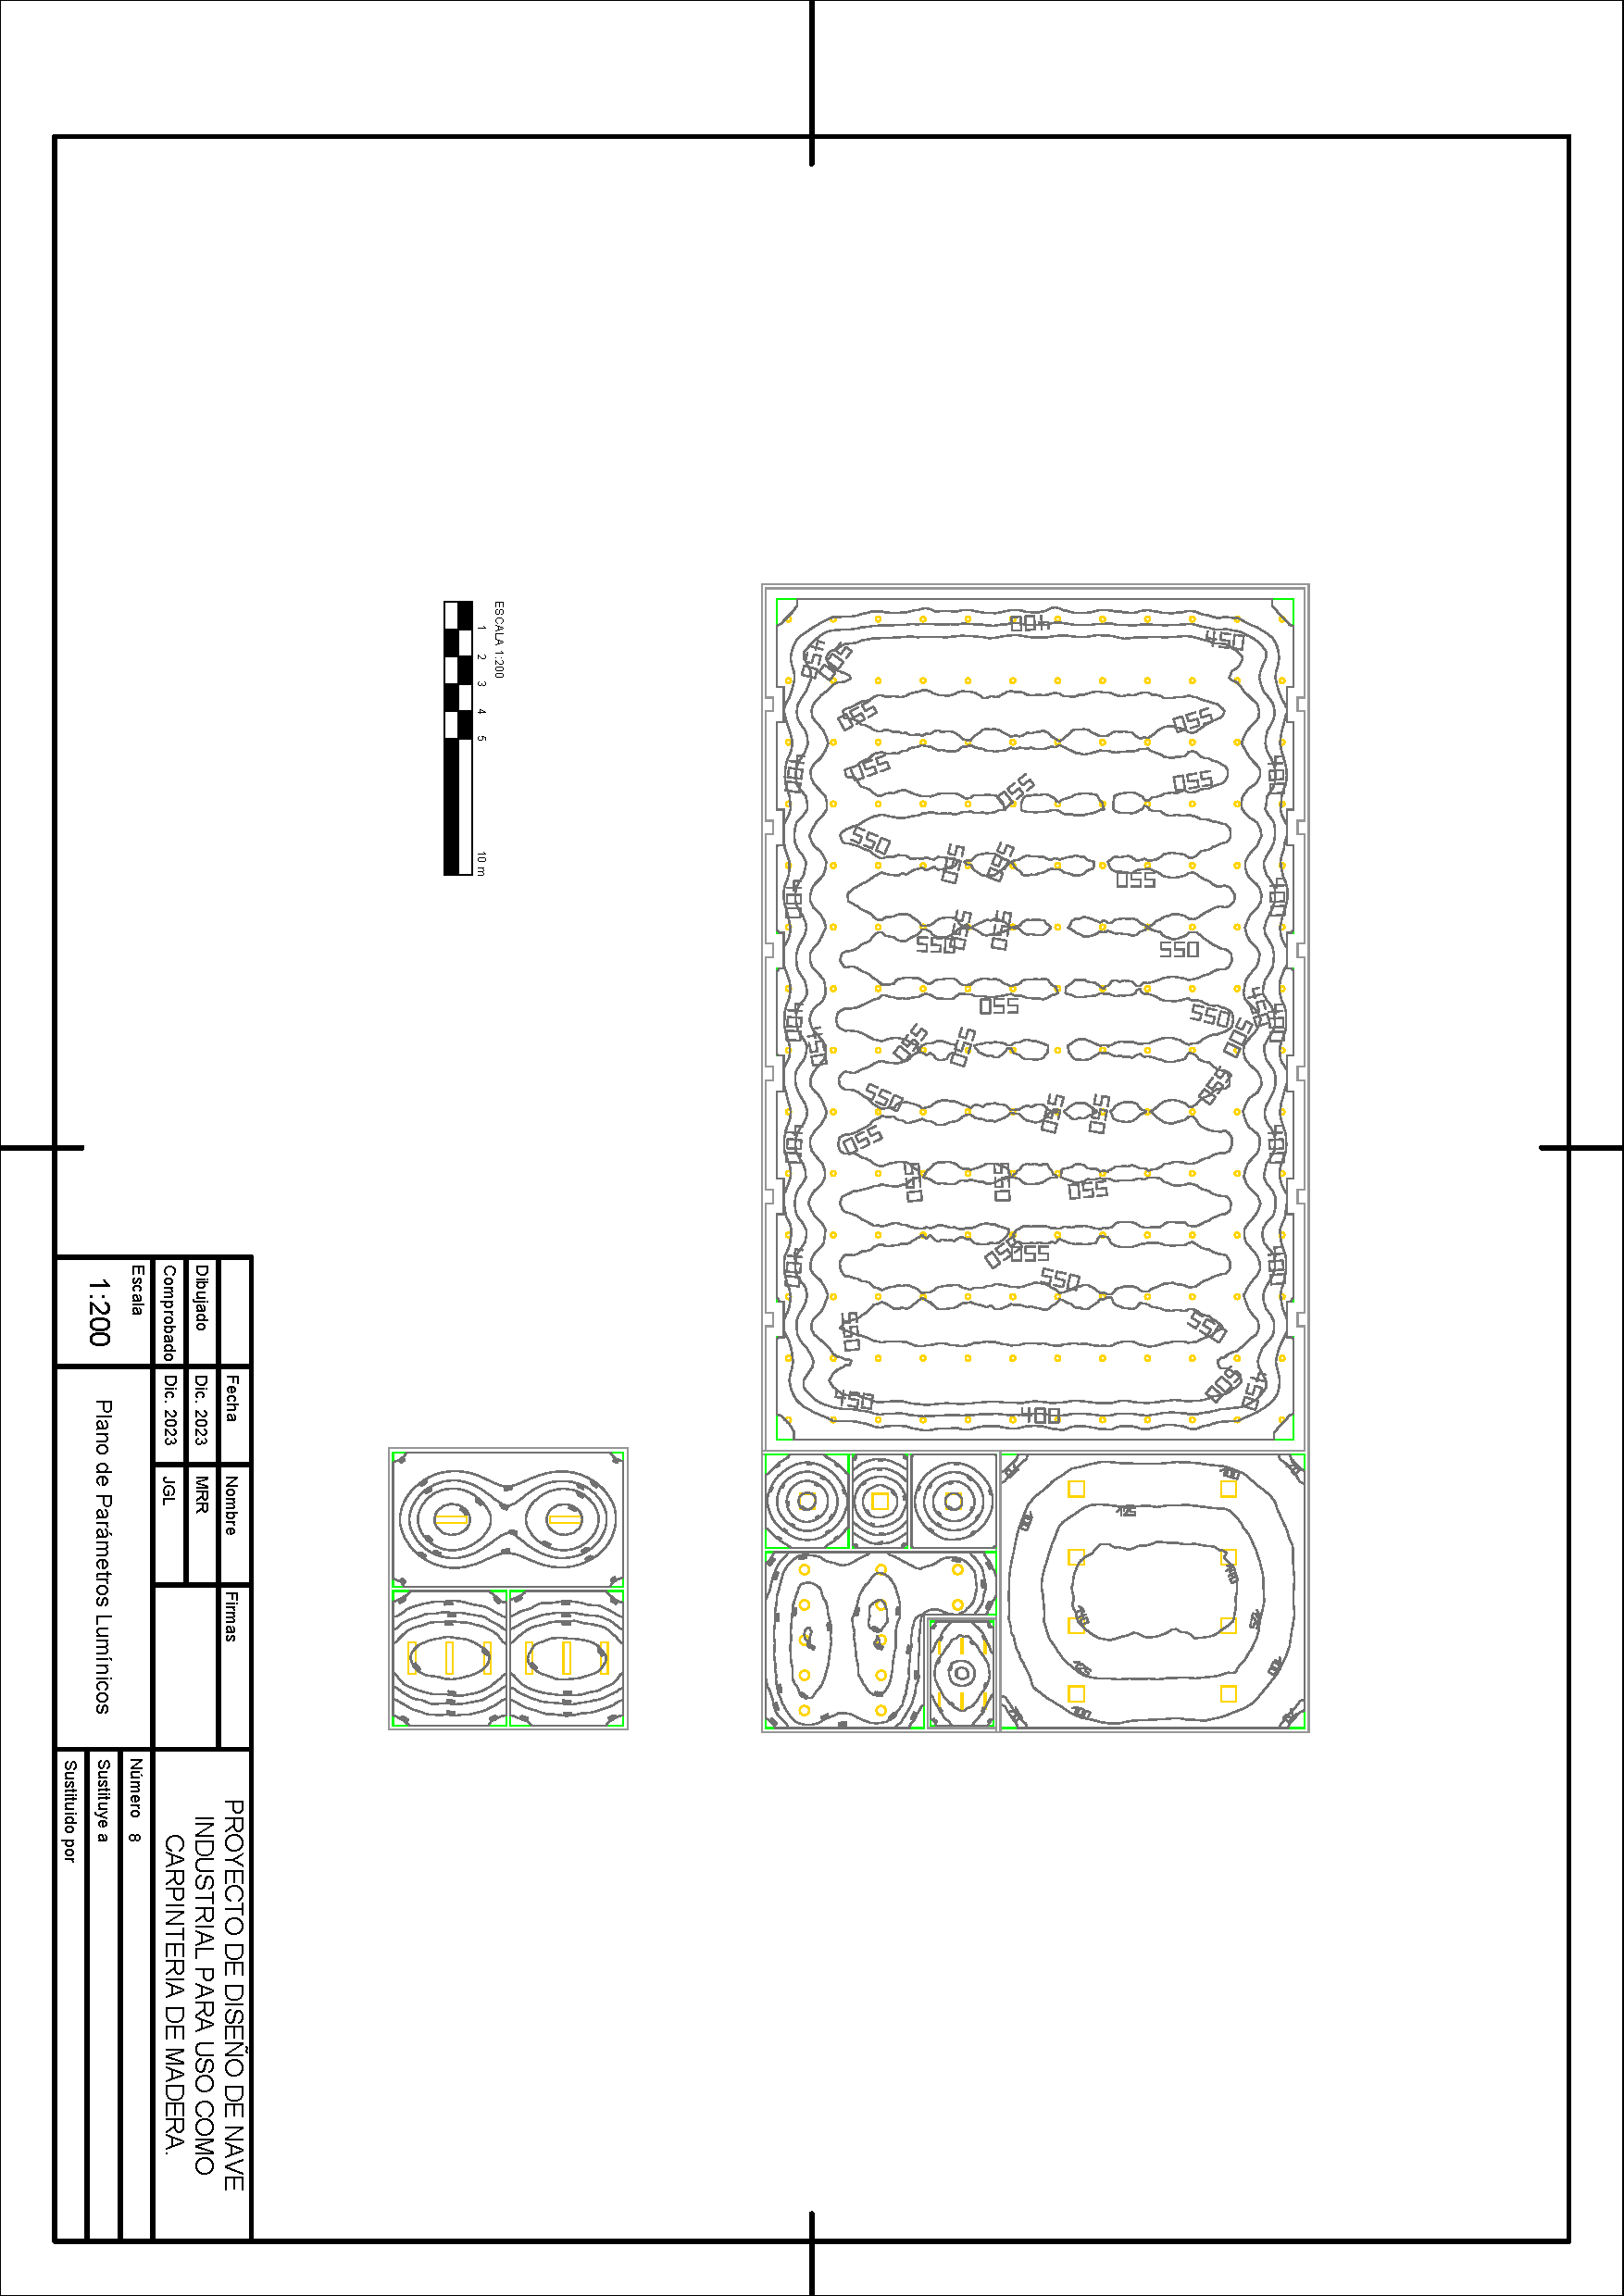
\includepdf[pages={1},pagecommand={
    \thispagestyle{empty}
    \addcontentsline{toc}{section}{Plano 8: Plano Instalación de Iluminación: Parámetros Lumínicos}}]{Planos/Plano Iluminacion.pdf}
    
% Circuitos eléctricos

% Esquema unifilar eléctrico
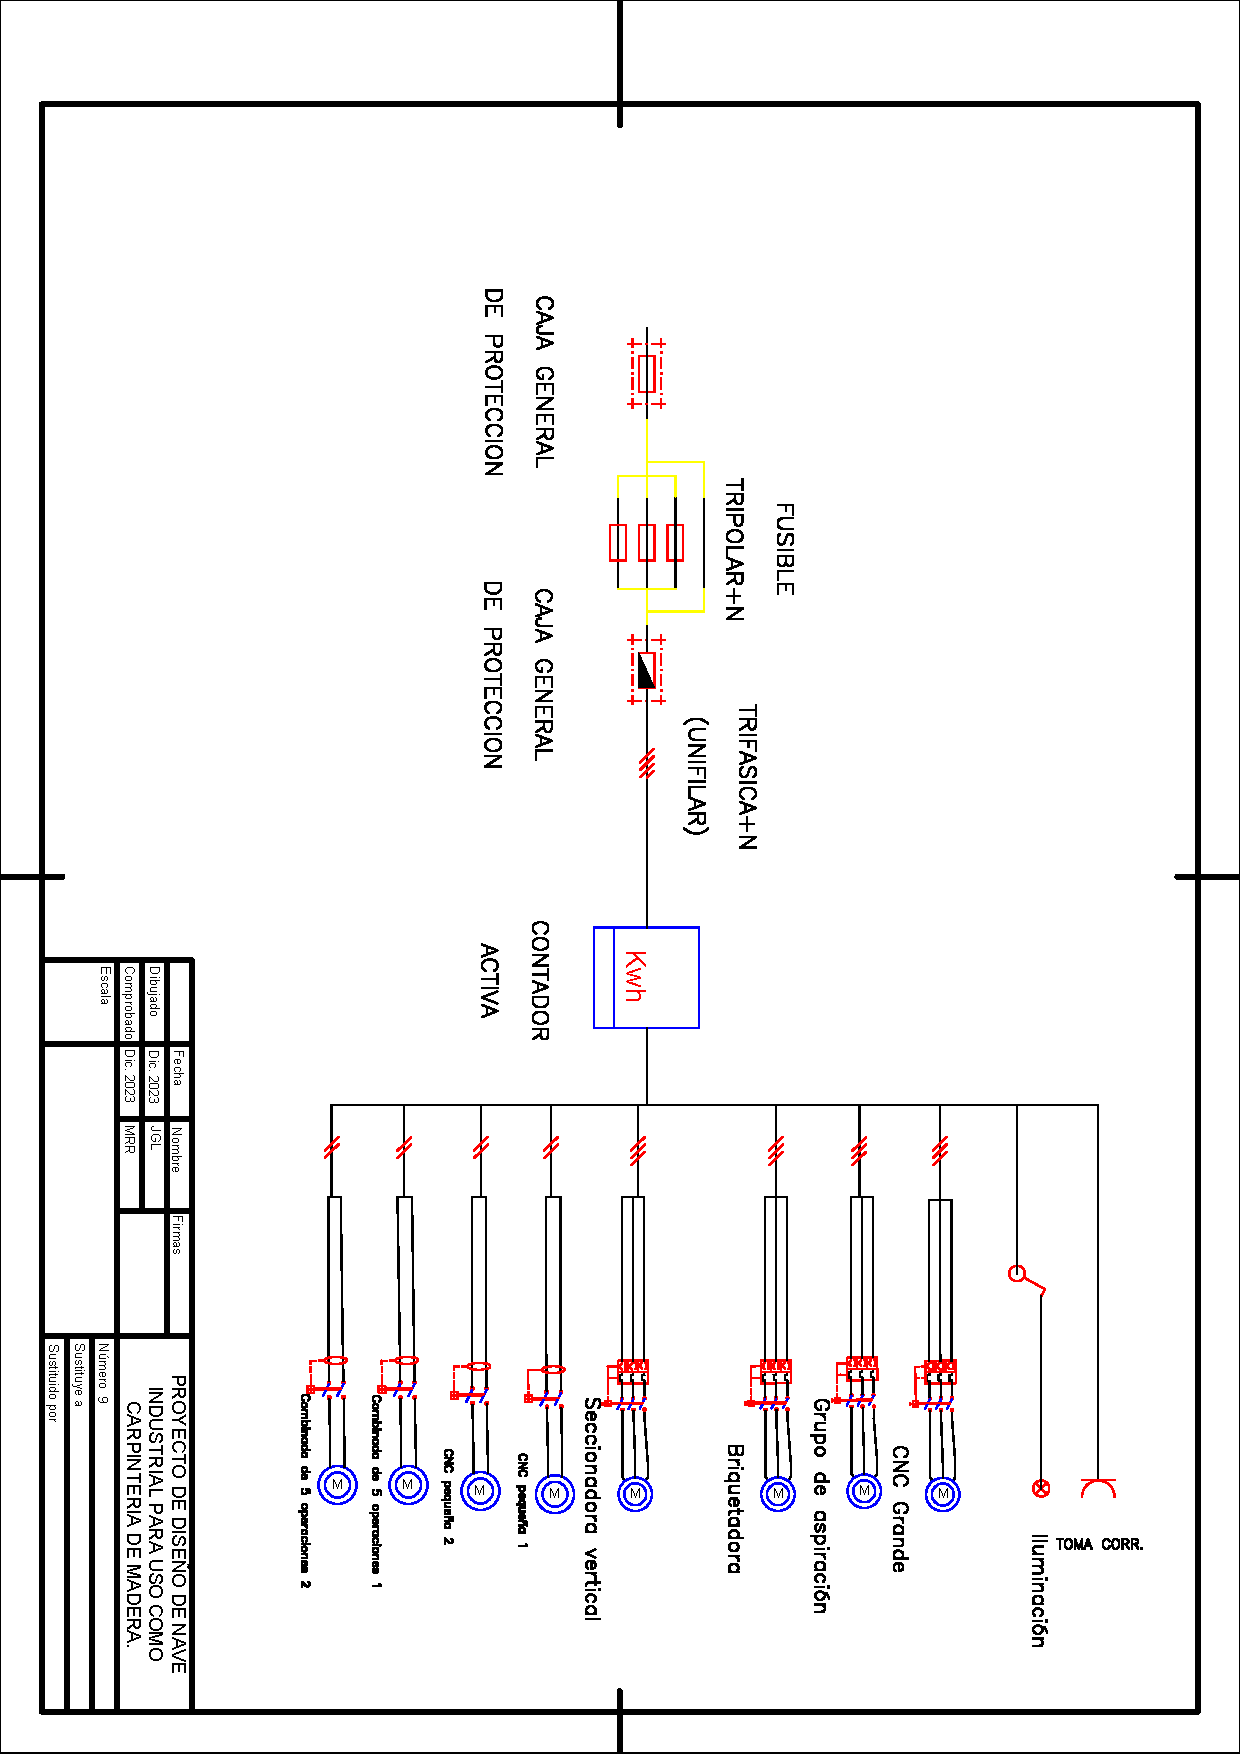
\includepdf[pages={1},pagecommand={
    \thispagestyle{empty}
    \addcontentsline{toc}{section}{Plano 9: Esquema Unifilar 1}}]{Planos/Unifilar1.pdf}

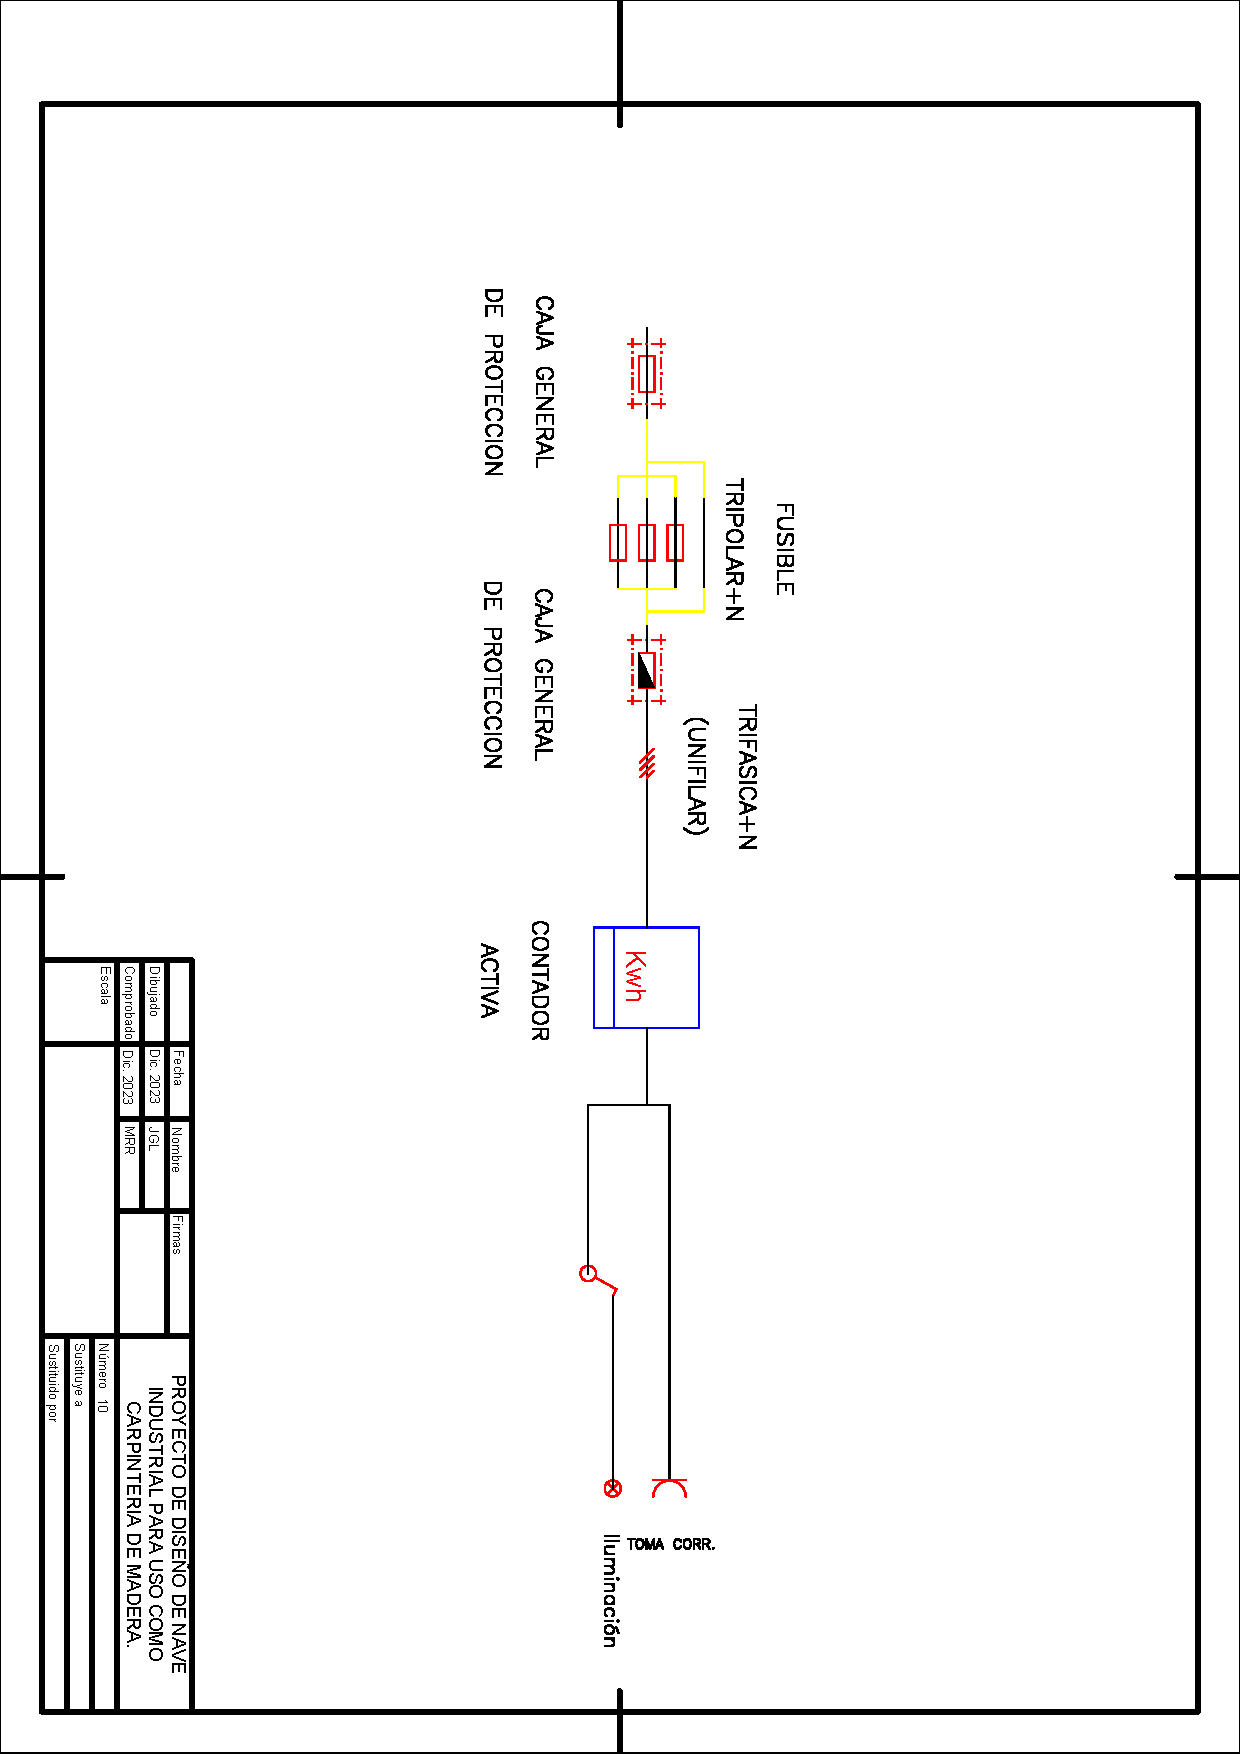
\includepdf[pages={1},pagecommand={
    \thispagestyle{empty}
    \addcontentsline{toc}{section}{Plano 10: Esquema Unifilar 2}}]{Planos/Unifilar2.pdf}

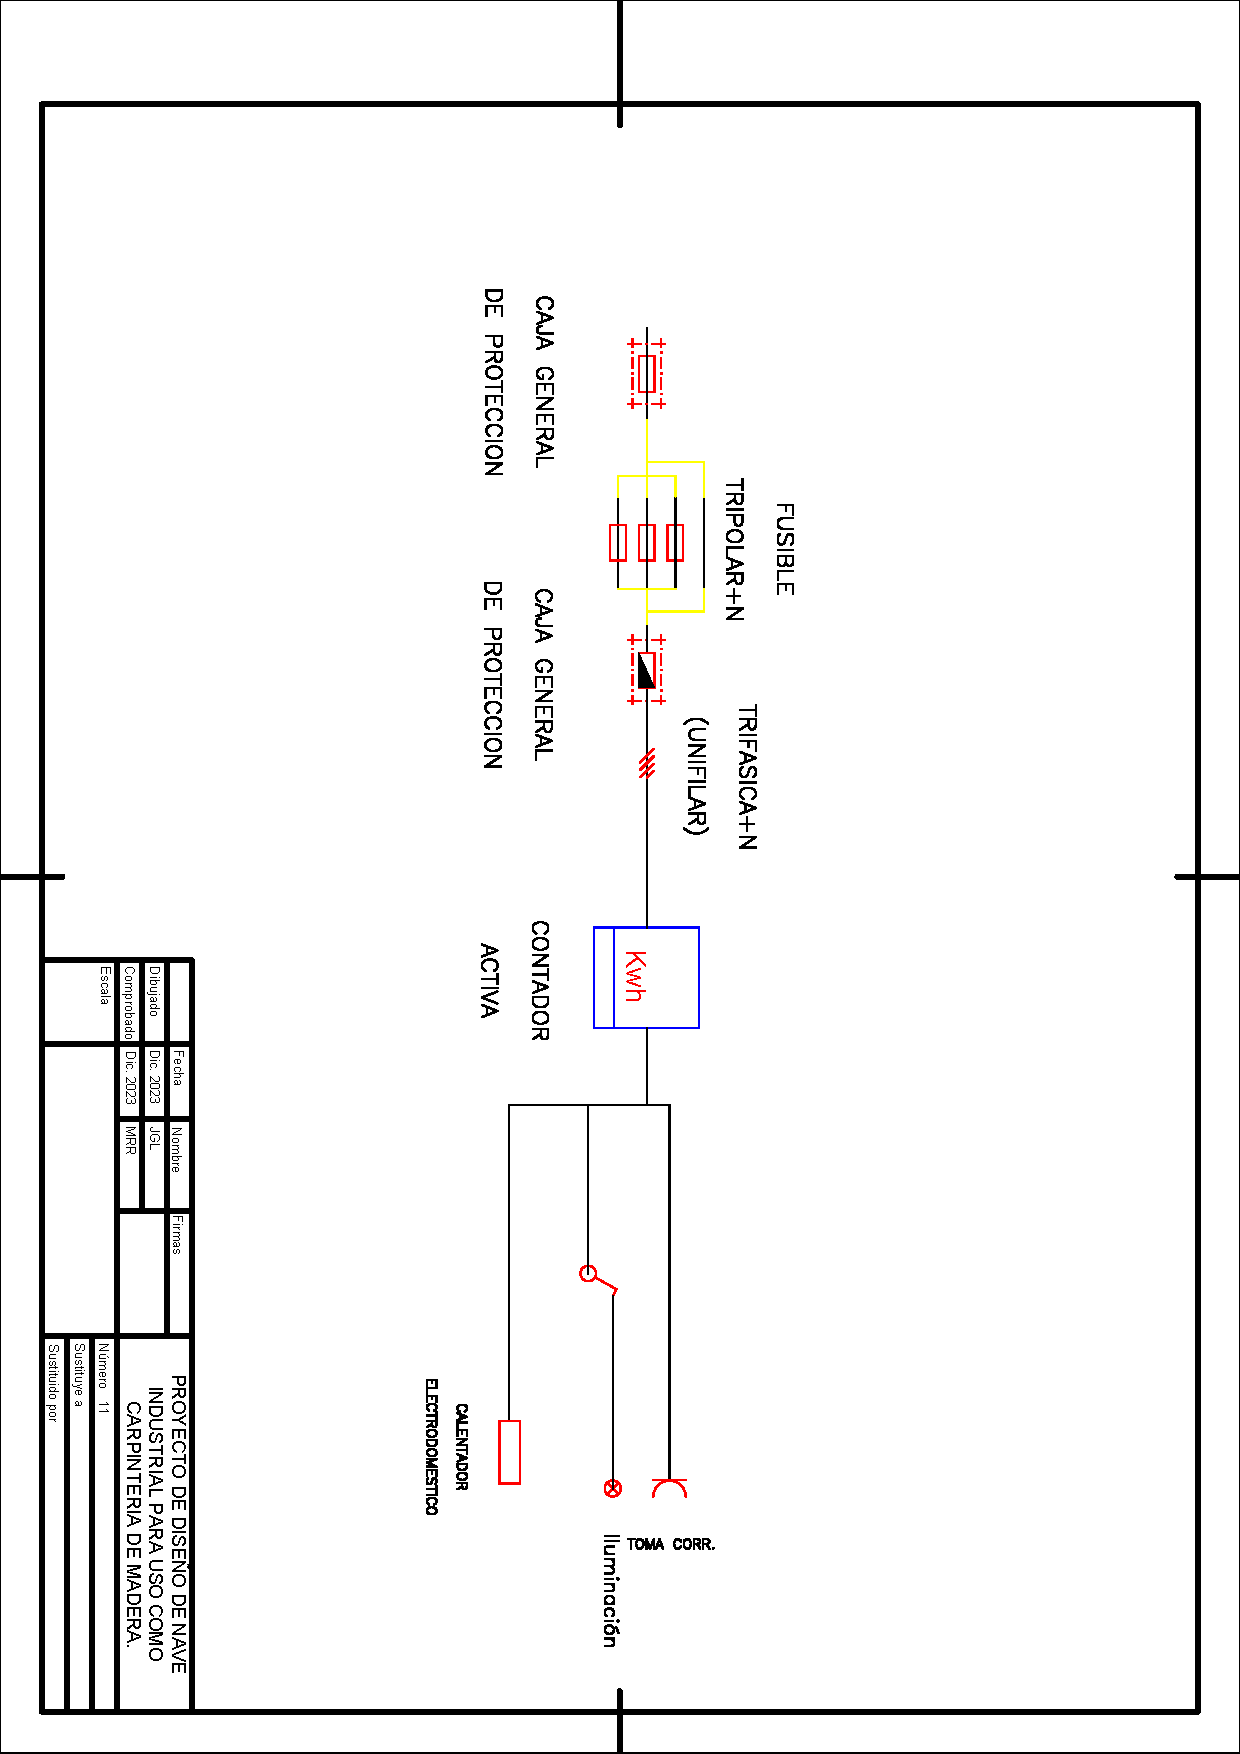
\includepdf[pages={1},pagecommand={
    \thispagestyle{empty}
    \addcontentsline{toc}{section}{Plano 11: Esquema Unifilar 3}}]{Planos/Unifilar3.pdf}
\toftagstop{Planos}
\end{document}